% Created 2019-12-20 Fri 09:38
% Intended LaTeX compiler: pdflatex
\documentclass[presentation,aspectratio=169,smaller]{beamer}
\usepackage[utf8x]{inputenc}
\usepackage[T1]{fontenc}
\usepackage{graphicx}
\usepackage{grffile}
\usepackage{longtable}
\usepackage{wrapfig}
\usepackage{rotating}
\usepackage[normalem]{ulem}
\usepackage{amsmath}
\usepackage{textcomp}
\usepackage{amssymb}
\usepackage{capt-of}
\usepackage{hyperref}
\usepackage{color}
\usepackage[newfloat]{minted}
\usepackage[utf8]{inputenc}
\usepackage{soul}
\usepackage{unicode-math}
\usepackage{mathtools}
\usepackage[mathletters]{ucs}
\usemintedstyle{tango}
\setminted{fontsize=\scriptsize}
\setminted{mathescape=true}
\setbeamertemplate{itemize items}[circle]
\setbeamertemplate{enumerate items}[default]
\setlength{\parskip}{\baselineskip}%
\setlength{\parindent}{0pt}%
\setbeamertemplate{navigation symbols}{}%remove navigation symbols
\newcommand{\hlyellow}[1]{\colorbox{yellow!50}{$\displaystyle#1$}}
\newcommand{\hlfancy}[2]{\sethlcolor{#1}\hl{#2}}
\usetheme{default}
\author{Boris Buliga}
\date{December 20, 2019}
\title{Befriending your Git}
\subtitle{or how to grow a centipede}
\hypersetup{
 pdfauthor={Boris Buliga},
 pdftitle={Befriending your Git},
 pdfkeywords={},
 pdfsubject={},
 pdfcreator={Emacs 26.3 (Org mode 9.2.6)}, 
 pdflang={English}}
\begin{document}

\maketitle
\newcommand{\mathcolorbox}[2]{%
  \begingroup
  \setlength{\fboxsep}{2pt}%
  \colorbox{#1}{$\displaystyle #2$}%
  \endgroup
}

\AtBeginSection[]{
  \begin{frame}
  \vfill
  \centering
  \begin{beamercolorbox}[sep=8pt,center,shadow=true,rounded=true]{title}
    \usebeamerfont{title}\insertsectionhead\par%
  \end{beamercolorbox}
  \vfill
  \end{frame}
}

\section*{Intro}
\label{sec:orgd1f55df}
\begin{frame}[label={sec:orgc9a8f76}]{Known story}
For several days God did something interesting.

On the sixth day God was like:

\begin{quote}
Let the earth bring forth the living creature after its kind, cattle, and
creeping thing, and beast of the earth after its kind.
\end{quote}

And God saw that it was good.
\end{frame}

\begin{frame}[label={sec:org5ed7572}]{Divine rest}
\pause

\begin{center}
\includegraphics[width=.9\linewidth]{images/creepy-centipede.png}
\end{center}
\end{frame}

\begin{frame}[label={sec:org1244901}]{Commonalities}
\begin{center}
\includegraphics[width=.9\linewidth]{images/torvalds.png}
\end{center}
\end{frame}

\begin{frame}[label={sec:org28e5190}]{About me}
\begin{columns}
\begin{column}{0.75\columnwidth}
\begin{itemize}
\item Server developer @Wix.
\item Haskell ↔ Emacs Lisp extremist. Whatever that means.
\item Chinese tea lover.
\item Wine-lifestyle activist (92\% of my life).
\end{itemize}
\end{column}

\begin{column}{0.25\columnwidth}
\begin{center}
\includegraphics[height=3.5cm]{images/boris.jpg}
\end{center}
\end{column}
\end{columns}
\end{frame}

\begin{frame}[label={sec:orgca57c1b}]{Agenda}
\begin{itemize}
\item What is Git
\item Initial setup
\item Commits
\item Branches
\item Stash
\item Merging
\item Rebasing
\item Undoing stuff
\end{itemize}
\end{frame}

\section{Version control systems}
\label{sec:org60879f1}

\begin{frame}[label={sec:org95ac4f1}]{Version Control}
Reasons to use:

\begin{enumerate}
\item A clear indicator of changes.
\item To know what is different between two versions of something.
\end{enumerate}

As a bonus - backup system.

Does it apply only to \alert{code}?
\end{frame}

\begin{frame}[label={sec:orgd99c47b}]{Tricky questions}
\begin{enumerate}
\item How to name revisions?
\begin{enumerate}
\item Date
\item Incremental number
\item Some magic hash
\item Wine grape varieties
\item Snowball I, Snowball II, \ldots{}, Snowball IX, \ldots{}
\end{enumerate}
\item How much to save?
\begin{enumerate}
\item Only the changed files? Leads to hard time viewing the whole project at
particular point of time.
\item Only the changes in files? The same as above plus doesn't work for
binaries.
\item The whole project. Leads to wasted disk space (not that critical now,
but\ldots{})
\end{enumerate}
\item Collaboration is a huge tricky question!
\end{enumerate}
\end{frame}

\section{3 Generations}
\label{sec:org8eb430c}

\begin{frame}[label={sec:org0ec5684}]{Generation I}
\begin{enumerate}
\item Collaboration via locks - only one person can edit specific file.
\item No networking.
\item One file at time operations.
\end{enumerate}

Examples: RCS, SCCS.
\end{frame}

\begin{frame}[label={sec:orga044fd1}]{Generation II}
\begin{itemize}
\item More permissive collaboration:
\begin{itemize}
\item No locks.
\item Users must merge current revision in order to commit changes.
\end{itemize}
\item Centralized networking:
\begin{itemize}
\item One source of truth.
\item Requires connection to server in order to perform any operations (like
commit changes, switch between revisions).
\item No need to store all revisions locally.
\item No need to have whole project copy (one can checkout specific directory and
work only on the part of the project).
\end{itemize}
\end{itemize}

Examples: CVS, Subversion.
\end{frame}

\begin{frame}[label={sec:orgf879c4c}]{Generation III}
\begin{itemize}
\item Separates getting changes and posting changes.
\item Distributed
\begin{itemize}
\item Every copy is a full copy of repository.
\item No connection is required for most of the operations (only fetch and push
require connection). Thus some operations are much faster.
\item Requires more disk space.
\end{itemize}
\end{itemize}

Examples: Git, Mercurial, Bazaar, Darcs.
\end{frame}

\begin{frame}[label={sec:orge78d12a}]{Git}
\begin{quote}
the system wasn't really designed, but grew organically

--- Junio Hamano (2011)
\end{quote}

\begin{quote}
Take Concurrent Versions System (CVS) as an example of what not to do; if in
doubt, make the exact opposite decision.

--- Linus Torvalds (2007)
\end{quote}

\begin{itemize}
\item Main goal -- ease Linux development.
\item Main focus -- features.
\item Git is not easy. By no means.
\item But it's really cool.
\end{itemize}
\end{frame}

\section{Working locally}
\label{sec:org1aafb1b}

\begin{frame}[label={sec:org99ef0f0},fragile]{Introducing ourselves}
 \begin{minted}[]{bash}
$ git config [--global] user.name "Ștefan cel Mare"
$ git config [--global] user.email "stefan-ten-ten@gov.md"
\end{minted}

\pause

Believe me, it's the hardest thing!

\begin{itemize}
\item People forget to do it.
\item Don't upset Ștefan and set your name and email.
\item It's useful in some scenarios.
\end{itemize}
\end{frame}

\begin{frame}[label={sec:org078c144},fragile]{Creating a repository}
 \begin{minted}[]{bash}
$ mkdir my-super-repo
$ cd my-super-repo
$ git init
$ ls -la
$ git status
On branch master

No commits yet

nothing to commit (create/copy files and use "git add" to track)

\end{minted}
\end{frame}

\begin{frame}[label={sec:org2912395},fragile]{Adding content}
 \begin{onlyenv}<1>
\begin{minted}[]{bash}
$ echo "# Git Workshop" > README.md
$ git status
On branch master

No commits yet

Untracked files:
  (use "git add <file>..." to include in what will be committed)
  README.md

nothing added to commit but untracked files present (use "git add" to track)
\end{minted}
\end{onlyenv}


\begin{onlyenv}<2>
\begin{center}
\includegraphics[width=.9\linewidth]{images/git-add-0.png}
\end{center}
\end{onlyenv}

\begin{onlyenv}<3>
\begin{minted}[]{bash}
$ git add README.md
$ git status
On branch master

No commits yet

Changes to be committed:
  (use "git rm --cached <file>..." to unstage)
  new file:   README.md
\end{minted}
\end{onlyenv}

\begin{onlyenv}<4>
\begin{center}
\includegraphics[width=.9\linewidth]{images/git-add-1.png}
\end{center}
\end{onlyenv}

\begin{onlyenv}<5>
\begin{minted}[]{bash}
$ git commit -m "add README file"
[master (root-commit) 88d0e08] add README file
 1 file changed, 1 insertion(+)
 create mode 100644 README.md

$ git status
On branch master
nothing to commit, working tree clean
\end{minted}
\end{onlyenv}

\begin{onlyenv}<6>
\begin{center}
\includegraphics[width=.9\linewidth]{images/git-add-2.png}
\end{center}
\end{onlyenv}
\end{frame}

\begin{frame}[label={sec:orgab2a086},fragile]{Editing content}
 \begin{onlyenv}<1>
\begin{minted}[]{bash}
$ echo "" >> README.md
$ echo "Using Git is fun, right?" >> README.md

$ git status
On branch master
Changes not staged for commit:
  (use "git add <file>..." to update what will be committed)
  (use "git restore <file>..." to discard changes in working directory)
  modified:   README.md

no changes added to commit (use "git add" and/or "git commit -a")
\end{minted}
\end{onlyenv}

\begin{onlyenv}<2>
\begin{center}
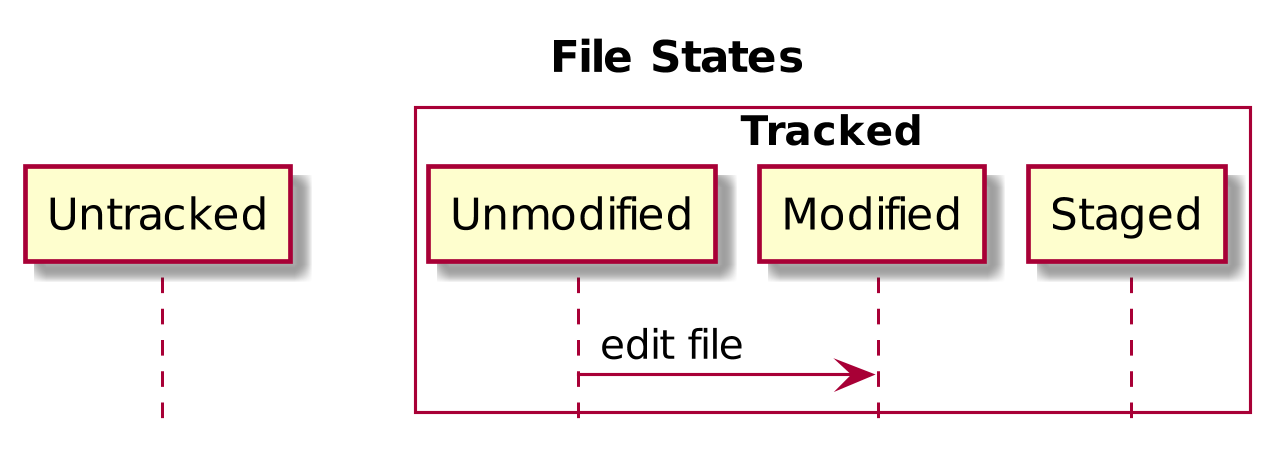
\includegraphics[width=.9\linewidth]{images/git-edit-0.png}
\end{center}
\end{onlyenv}

\begin{onlyenv}<3>
\begin{minted}[]{bash}
$ git add README.md

$ git status
On branch master
Changes to be committed:
  (use "git restore --staged <file>..." to unstage)
  modified:   README.md
\end{minted}
\end{onlyenv}

\begin{onlyenv}<4>
\begin{center}
\includegraphics[width=.9\linewidth]{images/git-edit-1.png}
\end{center}
\end{onlyenv}

\begin{onlyenv}<5>
\begin{minted}[]{bash}
$ git commit -m "update README file"
[master 7e29246] update README file
 1 file changed, 2 insertions(+)

$ git status
On branch master
nothing to commit, working tree clean
\end{minted}
\end{onlyenv}

\begin{onlyenv}<6>
\begin{center}
\includegraphics[width=.9\linewidth]{images/git-edit-2.png}
\end{center}
\end{onlyenv}
\end{frame}

\begin{frame}[label={sec:org24a4900},fragile]{Areas of Git}
 \begin{itemize}
\item Working directory - sandbox
\item Index (staging area) - proposed next commit snapshot
\item \texttt{.git} directory - repository database
\end{itemize}
\end{frame}

\begin{frame}[label={sec:org1ec375a}]{Areas of Git}
\begin{center}
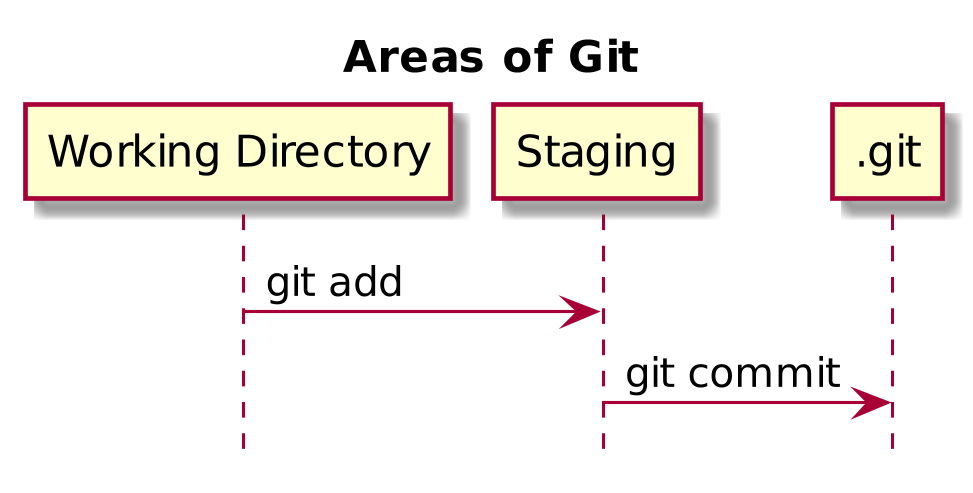
\includegraphics[width=.9\linewidth]{images/areas-of-git.png}
\end{center}
\end{frame}

\begin{frame}[label={sec:org11f5057},fragile]{Viewing commits}
 \begin{minted}[]{bash}
$ ls -l .git/objects

$ git log
\end{minted}
\end{frame}

\begin{frame}[label={sec:org0dff325},fragile]{Recap}
 \begin{itemize}
\item \texttt{git add}: add files to index (staging)
\item \texttt{git commit}: create a commit from staging
\item \texttt{git log}: list commits
\end{itemize}
\end{frame}

\section{A file system}
\label{sec:org9d3cb33}

\begin{frame}[label={sec:org5bd84ec},fragile]{What is commit}
 \begin{minted}[]{bash}
$ git show 7e29246
commit 7e2924627a293bf793e045d0b6ca1332f151afba (HEAD -> master)
Author: Boris Buliga <boris@d12frosted.io>
Date:   Sun Dec 15 19:20:29 2019 +0200

    update README file

diff --git a/README.md b/README.md
index 55a899f..dfdeab0 100644
--- a/README.md
+++ b/README.md
@@ -1 +1,3 @@
 # Git Workshop
+
+Using Git is fun, right?
\end{minted}
\end{frame}

\begin{frame}[label={sec:orgcbe6edb},fragile]{What is commit}
 \begin{minted}[]{bash}
$ git cat-file -t 7e29246
commit

$ git cat-file -p 7e29246
tree 43e7b8c24bc186e88becdeaaaa32c42a4a5c3a5b
parent 88d0e082f116578b6a815efe03372400c4456454
author Boris Buliga <boris@d12frosted.io> 1576430429 +0200
committer Boris Buliga <boris@d12frosted.io> 1576430429 +0200
gpgsig -----BEGIN PGP SIGNATURE-----

 iQIzBAABCAAdFiEEh3ycTfBYO6f60Is0+evwlDa8tQ8FAl32a10ACgkQ+evwlDa8
 ...
 ZVin9huB9mwAzGIyVOh/HONSt+QVnlGOtg8/mEKc7TFF7Mvjo/s=
 =RjUf
 -----END PGP SIGNATURE-----

update README file

$ λ git cat-file -p 43e7b8c24bc186e88becdeaaaa32c42a4a5c3a5b
100644 blob dfdeab0e7e7aeb6a8f639c386ed54d55a5b32988	README.md
\end{minted}
\end{frame}

\begin{frame}[label={sec:org0404b96}]{Three objects}
\begin{itemize}
\item Blobs
\item Trees
\item Commits
\end{itemize}
\end{frame}

\begin{frame}[label={sec:orge1bd294}]{Git is a file system}
\pause

\begin{center}
\includegraphics[height=6.7cm]{images/too-much.jpg}
\end{center}
\end{frame}

\begin{frame}[label={sec:orgc1fde27}]{But}
\begin{center}
\includegraphics[height=6.7cm]{images/what-is-branch.jpg}
\end{center}
\end{frame}

\section{Branches}
\label{sec:org06b3b7e}

\begin{frame}[label={sec:org0e369af},fragile]{Branch}
 \begin{minted}[]{bash}
$ cat .git/refs/heads/master
7e2924627a293bf793e045d0b6ca1332f151afba
\end{minted}

41 bytes (40 for hash and 1 for new line)

\pause

\begin{minted}[]{bash}
$ git cat-file -t 7e2924627a293bf793e045d0b6ca1332f151afba
commit

$ git cat-file -p 7e2924627a293bf793e045d0b6ca1332f151afba
tree 43e7b8c24bc186e88becdeaaaa32c42a4a5c3a5b
parent 88d0e082f116578b6a815efe03372400c4456454
author Boris Buliga <boris@d12frosted.io> 1576430429 +0200
committer Boris Buliga <boris@d12frosted.io> 1576430429 +0200
gpgsig -----BEGIN PGP SIGNATURE-----

 iQIzBAABCAAdFiEEh3ycTfBYO6f60Is0+evwlDa8tQ8FAl32a10ACgkQ+evwlDa8
 ...
 =RjUf
 -----END PGP SIGNATURE-----

update README file
\end{minted}
\end{frame}

\begin{frame}[label={sec:org344bd51},fragile]{Manipulating branches}
 \begin{itemize}
\item \texttt{git branch} - list the branches
\item \texttt{git branch NAME} - create a branch with \texttt{NAME}
\item \texttt{git branch -d NAME} - delete branch with \texttt{NAME}
\end{itemize}
\end{frame}

\begin{frame}[label={sec:org6f2d888},fragile]{Switching branches}
 \begin{center}
\begin{tabular}{lll}
action & pre 2.23 & post 2.23\\
\hline
switch to branch & \texttt{git checkout NAME} & \texttt{git switch NAME}\\
create and switch & \texttt{git checkout -b NAME} & \texttt{git switch -c NAME}\\
\end{tabular}
\end{center}
\end{frame}

\begin{frame}[label={sec:orgd96de04}]{Visualisation}
\begin{center}
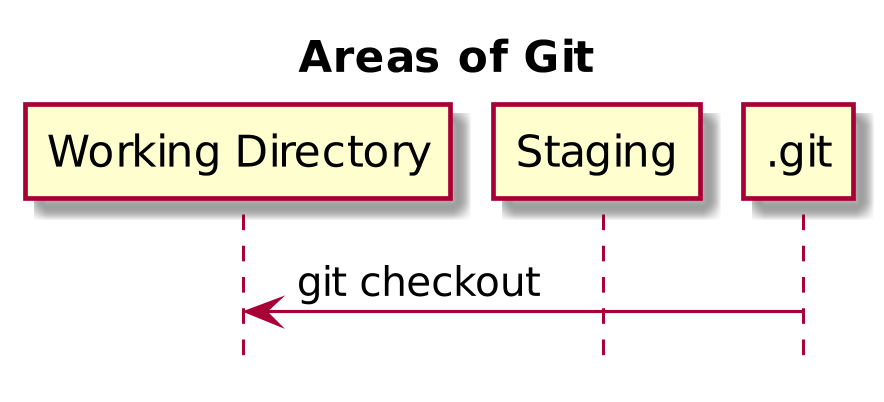
\includegraphics[height=6.7cm]{images/git-checkout-0.png}
\end{center}
\end{frame}

\begin{frame}[label={sec:orgf4605d7},fragile]{HEAD}
 \begin{itemize}
\item HEAD is a pointer of where current working directory is.
\begin{itemize}
\item \texttt{\$ cat .git/HEAD} prints the reference
\end{itemize}
\item HEAD is the last commit snapshot and the next parent.
\end{itemize}
\end{frame}

\begin{frame}[label={sec:org1e2aa27}]{Visualisation}
\begin{onlyenv}<1>
\begin{center}
\includegraphics[height=6.7cm]{images/head-0.png}
\end{center}

\scriptsize{https://git-scm.com/book/en/v2}
\end{onlyenv}

\begin{onlyenv}<2>
\begin{center}
\includegraphics[height=6.7cm]{images/head-1.png}
\end{center}

\scriptsize{https://git-scm.com/book/en/v2}
\end{onlyenv}

\begin{onlyenv}<3>
\begin{center}
\includegraphics[height=6.7cm]{images/head-2.png}
\end{center}

\scriptsize{https://git-scm.com/book/en/v2}
\end{onlyenv}

\begin{onlyenv}<4>
\begin{center}
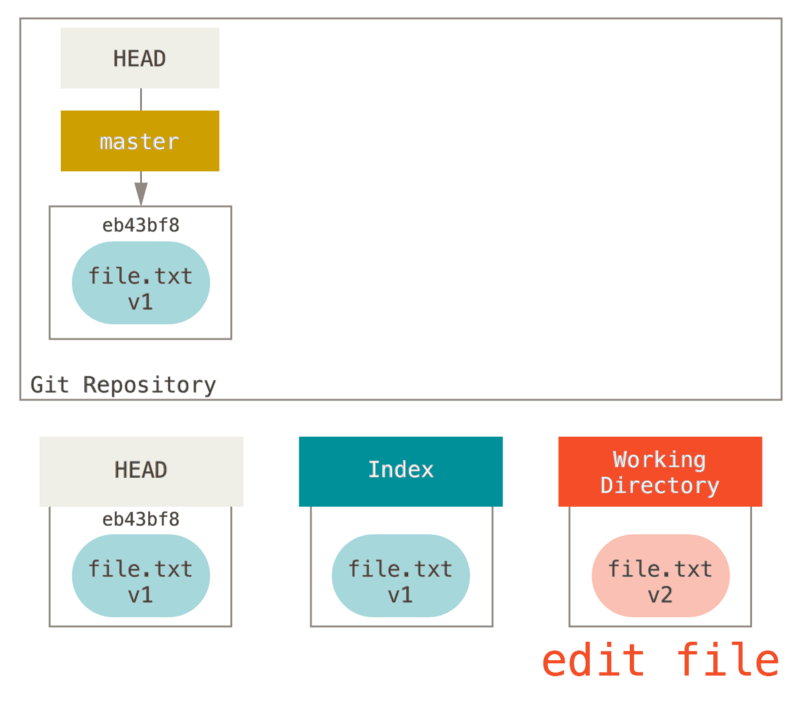
\includegraphics[height=6.7cm]{images/head-3.png}
\end{center}

\scriptsize{https://git-scm.com/book/en/v2}
\end{onlyenv}

\begin{onlyenv}<5>
\begin{center}
\includegraphics[height=6.7cm]{images/head-4.png}
\end{center}

\scriptsize{https://git-scm.com/book/en/v2}
\end{onlyenv}

\begin{onlyenv}<6>
\begin{center}
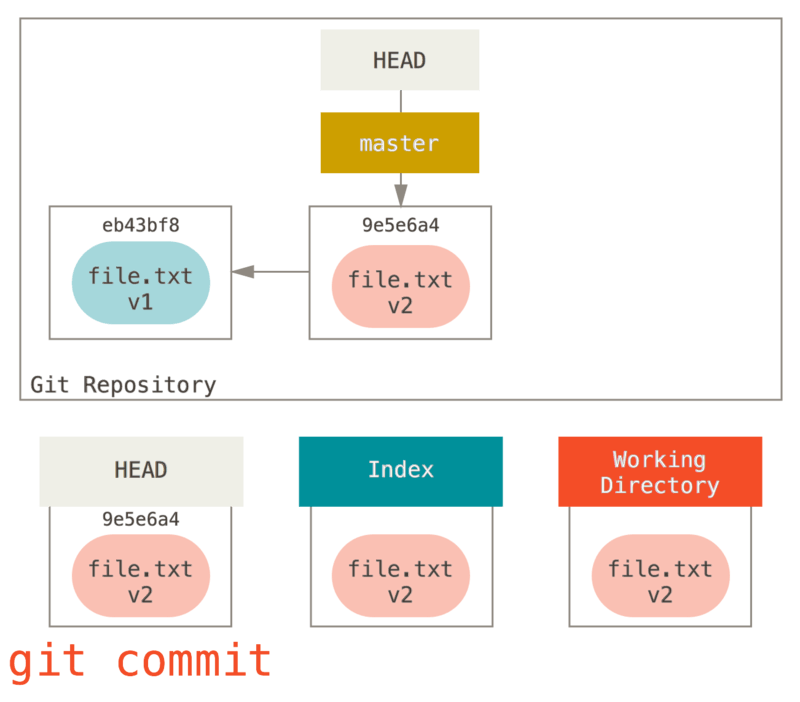
\includegraphics[height=6.7cm]{images/head-5.png}
\end{center}

\scriptsize{https://git-scm.com/book/en/v2}
\end{onlyenv}
\end{frame}

\begin{frame}[label={sec:org5a6f818},fragile]{Switching to commit}
 \begin{columns}
\begin{column}[t]{0.46\columnwidth}
\begin{minted}[]{bash}
$ git checkout 88d0e08
Note: switching to '88d0e08'.

You are in 'detached HEAD' state. You can look around,
make experimental changes and commit them, and you can
discard any commits you make in this state without
impacting any branches by switching back to a branch.

If you want to create a new branch to retain commits
you create, you may do so (now or later) by using -c
with the switch command. Example:

  git switch -c <new-branch-name>

Or undo this operation with:

  git switch -

Turn off this advice by setting config variable
advice.detachedHead to false

HEAD is now at 88d0e08 add README file
\end{minted}
\end{column}

\begin{column}[t]{0.46\columnwidth}
\begin{minted}[]{bash}
$ git switch 88d0e08
fatal: a branch is expected, got commit '88d0e08'

$ git switch --detach 88d0e08
HEAD is now at 88d0e08 add README file
\end{minted}
\end{column}
\end{columns}
\end{frame}

\begin{frame}[label={sec:orge811c3b},fragile]{Dealing with detached HEAD}
 \begin{onlyenv}<1>
After you make a commit on detached \texttt{HEAD}:

\begin{minted}[]{bash}
λ git lg master HEAD
* 864a083 <Boris Buliga> - (HEAD, detached-head-file) detached head file (2 minutes ago)
| * efd7f07 <Boris Buliga> - (master) add game.exe (32 hours ago)
| * 7e29246 <Boris Buliga> - (feature/whatever) update README file (3 days ago)
|/
* 88d0e08 <Boris Buliga> - add README file (3 days ago)
\end{minted}
\end{onlyenv}

\begin{onlyenv}<2>
\begin{minted}[]{bash}
$ git checkout master
Previous HEAD position was 864a083 detached head file
Switched to branch 'master'

$ git cherry-pick 864a083
[master 2aacafb] detached head file
 Date: Wed Dec 18 16:10:41 2019 +0200
 1 file changed, 0 insertions(+), 0 deletions(-)
 create mode 100644 detached-head-file

$ git lg
* 2aacafb <Boris Buliga> - (HEAD -> master) detached head file (2 seconds ago)
* efd7f07 <Boris Buliga> - add game.exe (32 hours ago)
* 7e29246 <Boris Buliga> - (feature/whatever) update README file (3 days ago)
* 88d0e08 <Boris Buliga> - add README file (3 days ago)
\end{minted}
\end{onlyenv}

\begin{onlyenv}<3>
\begin{minted}[]{bash}
$ git branch detached-head-file

$ git checkout master
Previous HEAD position was 864a083 detached head file
Switched to branch 'master'

$ git merge detached-head-file
Merge made by the 'recursive' strategy.
 detached-head-file | 0
 1 file changed, 0 insertions(+), 0 deletions(-)
 create mode 100644 detached-head-file

$ git lg
*   7e24cc1 <Boris Buliga> - (HEAD -> master) Merge branch 'detached-head-file' (5 seconds ago)
|\
| * 864a083 <Boris Buliga> - (detached-head-file) detached head file (4 minutes ago)
* | efd7f07 <Boris Buliga> - add game.exe (32 hours ago)
* | 7e29246 <Boris Buliga> - (feature/whatever) update README file (3 days ago)
|/
* 88d0e08 <Boris Buliga> - add README file (3 days ago)
\end{minted}
\end{onlyenv}
\end{frame}

\begin{frame}[label={sec:org8d5da12}]{How it looked}
\begin{center}
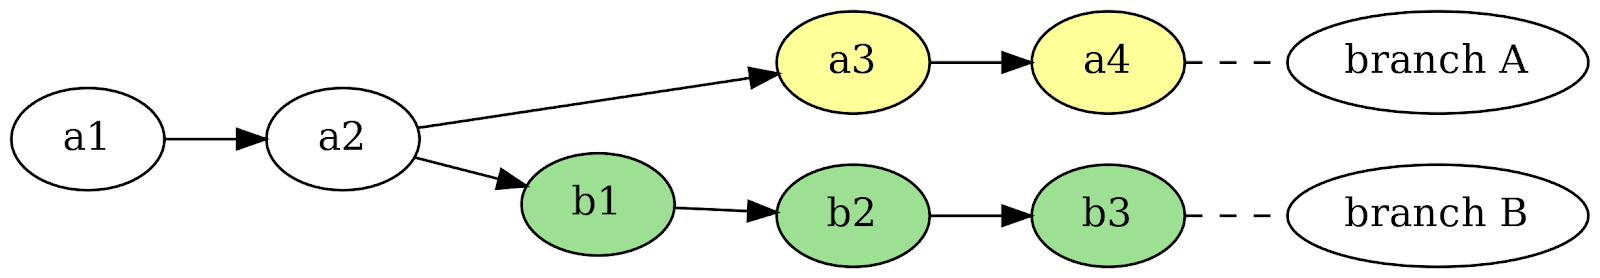
\includegraphics[width=.9\linewidth]{images/merging-vs-rebasing-0.png}
\end{center}
\end{frame}

\begin{frame}[label={sec:org19ef3f4},fragile]{After merge}
 \begin{minted}[]{bash}
$ git checkout branch-a
$ git merge branch-b
\end{minted}

\begin{center}
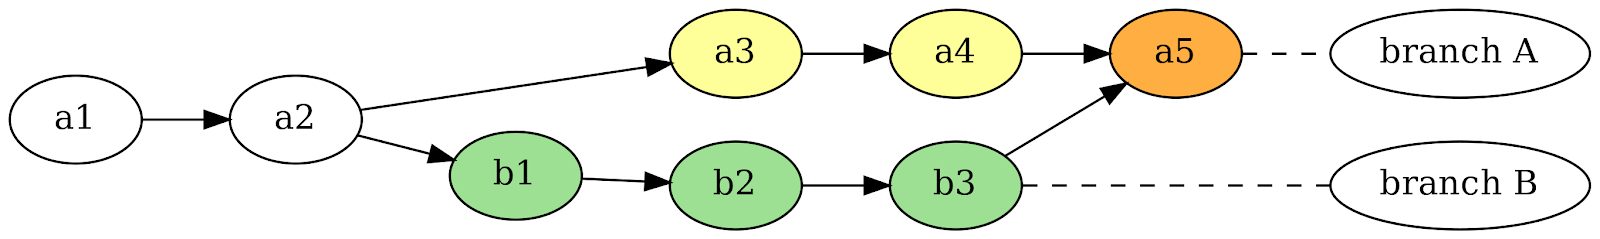
\includegraphics[width=.9\linewidth]{images/merging-vs-rebasing-1.png}
\end{center}
\end{frame}

\begin{frame}[label={sec:orgd4b46cb}]{How it looked}
\begin{center}
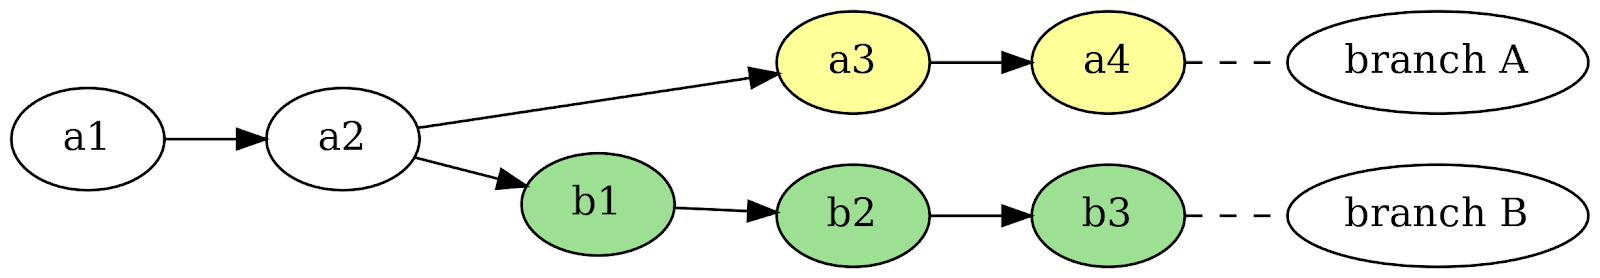
\includegraphics[width=.9\linewidth]{images/merging-vs-rebasing-0.png}
\end{center}
\end{frame}


\begin{frame}[label={sec:org040223a},fragile]{After rebase}
 \begin{minted}[]{bash}
$ git checkout branch-b
$ git rebase branch-a
\end{minted}

\begin{center}
\includegraphics[width=.9\linewidth]{images/merging-vs-rebasing-2.png}
\end{center}
\end{frame}

\begin{frame}[label={sec:org0e73213},fragile]{After rebase + merge}
 \begin{minted}[]{bash}
$ git checkout branch-a
$ git merge branch-b
\end{minted}

\begin{center}
\includegraphics[width=.9\linewidth]{images/merging-vs-rebasing-2.png}
\end{center}
\end{frame}

\begin{frame}[label={sec:org1402284}]{Working with conflicts}
Fieldwork
\end{frame}

\begin{frame}[label={sec:orgf7c305d},fragile]{Aborting}
 \begin{minted}[]{bash}
$ git merge --abort
$ git rebase --abort
$ git cherry-pick --abort
\end{minted}
\end{frame}

\section{Undoing stuff}
\label{sec:org3b8d19a}

\begin{frame}[label={sec:orge6de410}]{Reset}
\begin{center}
\includegraphics[height=6.7cm]{images/reset-start.png}
\end{center}

\scriptsize{https://git-scm.com/book/en/v2}
\end{frame}

\begin{frame}[label={sec:org6ea2562}]{Three levels of reset}
\begin{itemize}
\item Soft reset
\item Mixed reset (mixed feelings is what you get)
\item Hard reset
\end{itemize}
\end{frame}

\begin{frame}[label={sec:orgb236308}]{Hard reset}
\begin{center}
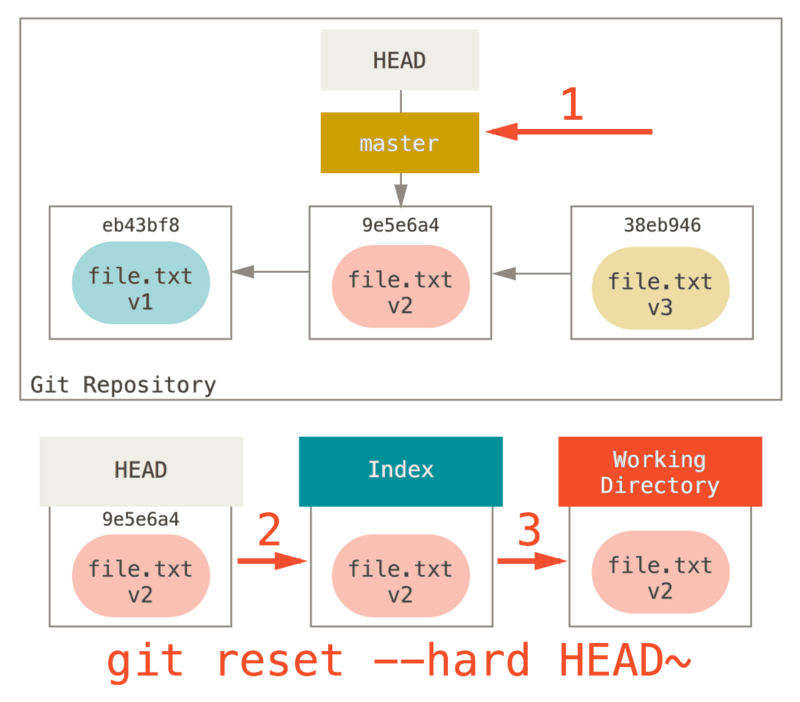
\includegraphics[height=6.7cm]{images/reset-hard.png}
\end{center}

\scriptsize{https://git-scm.com/book/en/v2}
\end{frame}

\begin{frame}[label={sec:org1397e9c}]{Mixed reset}
\begin{center}
\includegraphics[height=6.7cm]{images/reset-mixed.png}
\end{center}

\scriptsize{https://git-scm.com/book/en/v2}
\end{frame}

\begin{frame}[label={sec:org23a9a69}]{Soft reset}
\begin{center}
\includegraphics[height=6.7cm]{images/reset-soft.png}
\end{center}

\scriptsize{https://git-scm.com/book/en/v2}
\end{frame}

\begin{frame}[label={sec:orgd03a934}]{Checkout}
\begin{center}
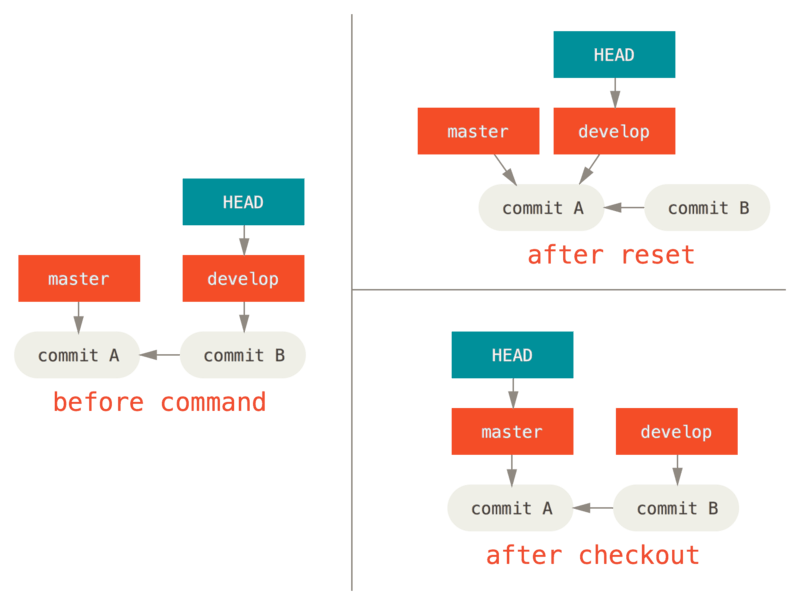
\includegraphics[height=6.7cm]{images/reset-checkout.png}
\end{center}

\scriptsize{https://git-scm.com/book/en/v2}
\end{frame}

\section{Stash}
\label{sec:org426cddd}

\section{Collaboration}
\label{sec:orgd2a0548}

\begin{frame}[label={sec:orgcfd8e0e}]{Collaboration}
\begin{itemize}
\item remotes
\item fetching
\item pushing
\item cloning
\end{itemize}
\end{frame}

\begin{frame}[label={sec:orgc52aa56}]{Collaboration}
\begin{itemize}
\item Patches
\item Pull requests
\item Reviews
\end{itemize}
\end{frame}

\section*{References}
\label{sec:org9c915f7}
\begin{frame}[label={sec:org250b40f},fragile]{References}
 \begin{itemize}
\item \texttt{man git <command>}
\item Pro Git: \url{https://git-scm.com/book/en/v2}
\item \url{https://github.blog/2019-08-16-highlights-from-git-2-23/}
\item \url{https://redfin.engineering/two-commits-that-wrecked-the-user-experience-of-git-f0075b77eab1}
\end{itemize}
\end{frame}

\section{Questions?}
\label{sec:org8d3a751}
\section{Thank you}
\label{sec:org8616cca}
\end{document}
